%% ***************************************************************************
%% My paper
%%
%% Authors: Emmett Brown, Marty McFly, Biff Tannen
%%
%% NOTE: this file will not compile until you called the script
%% generate-preamble.php once. See the file Readme.md to understand what
%% to do.
%%
%% This paper is an instance of the PaperShell template. For more
%% information, please visit https://github.com/sylvainhalle/PaperShell
%% ***************************************************************************
%% ---------------------------
%% Author preamble. The contents of this file change depending on the
%% paper class you choose.
%% ---------------------------
  
%%%%%%%%%%%%%%%%%%%%%%%%%%%%%%%%%%%%%%%%%%%%%%%%%%%%%%%%%%%%%%%%%%%%%%%%%%
%% This file was autogenerated by PaperShell v2.6.1 on 2023-02-03 13:51:10
%% https://github.com/sylvainhalle/PaperShell
%% DO NOT EDIT!
%%%%%%%%%%%%%%%%%%%%%%%%%%%%%%%%%%%%%%%%%%%%%%%%%%%%%%%%%%%%%%%%%%%%%%%%%%
\documentclass[preprint]{elsarticle}

% Usual packages
\usepackage[utf8]{inputenc}  % UTF-8 input encoding
\usepackage[T1]{fontenc}     % Type1 fonts
\usepackage{lmodern}         % Improved Computer Modern font
\usepackage{microtype}       % Better handling of typo
\usepackage[scaled]{helvet} % Scale Helvetica
\usepackage[english]{babel}  % Hyphenation
\usepackage{graphicx}        % Import graphics
\usepackage[bookmarks=false]{hyperref}            % Better handling of references in PDFs
\usepackage{comment}         % To comment out blocks of text
\biboptions{sort&compress}   % Sort and compress citations

\journal{TISSEC}

% User-defined includes
%% ---------------------------
%% If you have other packages or command definitions you'd like to
%% include, write them there
%% ---------------------------
\usepackage{amsmath,amsfonts,amssymb}

%% Note: the subfig package is incompatible with the "unfixed" version
%% of the LIPICS class. It works here only because PaperShell includes
%% a fixed version --which is not the official version.
\usepackage{subfig}

%% We put one here: this is a dummy command for LaTeX, used to
%% tell Aspell to skip checking the spelling of what's inside
%% Usage: I like the word \nospellcheck{kwyjibo}
\newcommand{\nospellcheck}[1]{#1}

%% --------------------------
%% Personalized todo notes
%% --------------------------
\usepackage{xcolor}
\usepackage{todonotes}
%\newcommand{\todosylvain}[1]{\todo[inline,caption={},color=cyan]{\sf\small \textbf{@Sylvain:} #1}}
%\newcommand{\todoalex}[1]{\todo[inline,caption={},color=pink]{\sf\small \textbf{@Alex:} #1}}
%\newcommand{\todosebastien}[1]{\todo[inline,caption={},color=lime]{\sf\small \textbf{@Sébastien:} #1}}
%\newcommand{\todomichael}[1]{\todo[inline,caption={},color=lime]{\sf\small \textbf{@Michaël:} #1}}
%\newcommand{\todotous}[1]{\todo[inline,caption={},color=yellow]{\sf\small #1}}
%\newcommand{\todoedmond}[1]{\todo[inline,caption={},color=lime]{\sf\small \textbf{@Edmond:} #1}}

%% --------------------------
%% Placeholder for figure
%% --------------------------
\newcommand{\imagevide}{\framebox(200,200){IMAGE}}

%% --------------------------
%% Alter some LaTeX defaults for better treatment of figures:
%% See p.105 of "TeX Unbound" for suggested values.
%% See pp. 199-200 of Lamport's "LaTeX" book for details.
%% --------------------------
%% Parameters for all pages
\renewcommand{\topfraction}{0.9}	% max fraction of floats at top
\renewcommand{\bottomfraction}{0.8}	% max fraction of floats at bottom

%% Parameters for TEXT pages (not float pages)
\setcounter{topnumber}{2}
\setcounter{bottomnumber}{2}
\setcounter{totalnumber}{4}                 % 2 may work better
\setcounter{dbltopnumber}{2}                % for 2-column pages
\renewcommand{\dbltopfraction}{0.9}         % fit big float above 2-col. text
\renewcommand{\textfraction}{0.07}          % allow minimal text w. figs

% Parameters for FLOAT pages (not text pages)
\renewcommand{\floatpagefraction}{0.7}      % require fuller float pages
% N.B.: floatpagefraction MUST be less than topfraction !!
\renewcommand{\dblfloatpagefraction}{0.7}   %require fuller float pages

%\newtheorem{example}{Example}
%% Default path for graphics
\graphicspath{{fig/}}


\begin{document}

\begin{frontmatter}

% Title
\title{Applications of the Flux Capacitor}

% Authors and affiliations
\author{Emmett Brown\fnref{label1}%
}
\author{Marty McFly\fnref{label1}%
}
\author{Biff Tannen\fnref{label2}%
}
\fntext[label1]{Temporal Industries, Hill Valley, CA 95420%
}
\fntext[label2]{BiffCo inc., Hill Valley, CA 95420%
}
\begin{abstract}
%% ----------------------
%% Write your abstract here. Do not enclose it in an "abstract"
%% environment.
%% ----------------------
Lorem ipsum dolor sit amet, consectetur adipiscing elit. Quisque rhoncus auctor mauris. Vestibulum ante ipsum primis in faucibus orci luctus et ultrices posuere cubilia Cur\ae{}; Sed a metus nec felis tristique venenatis eu quis urna. Integer quis sagittis eros, condimentum auctor libero. Fusce luctus diam et libero sodales luctus. Duis suscipit sodales libero, sed blandit odio aliquam at. Sed venenatis orci et luctus sagittis. Nam aliquam mi mi, ut vehicula turpis semper at. Nam pellentesque est nec fringilla consectetur. Aliquam magna elit, imperdiet et condimentum nec, venenatis et nisi. 
%% :folding=explicit:wrap=soft:mode=latex:

\end{abstract}
\end{frontmatter}


%% ---------------------------
%% If you wish to include additional packages, define new environments or
%% new commands, put them in the file includes.tex
%%
%% Write your abstract in the file abstract.tex.
%% ---------------------------

%% ---------------------------
%% Introduction
%% ---------------------------
\section{Introduction} %% {{{

M\ae{}cenas sodales ex in risus convallis elementum. Pr\ae{}sent at sem fermentum, egestas dolor non, ultrices elit. Cras at justo sit amet dolor lobortis blandit. Phasellus sodales erat eget tellus facilisis tristique. Nulla purus velit, hendrerit in cursus ut, euismod vit\ae{} odio. Morbi nec metus quis augue interdum ullamcorper ac at nisi. Nullam vit\ae{} imperdiet mauris. Nullam a ligula felis. Etiam at erat blandit nibh interdum posuere id at mi. Ut vit\ae{} ornare leo. Morbi vestibulum mauris id tellus volutpat, eget feugiat lorem maximus.

Donec maximus dui quis velit placerat auctor. Fusce vel tincidunt mi, vel porta eros. Fusce egestas purus sit amet ex hendrerit, at commodo justo rutrum. Nam interdum pharetra commodo. Duis ligula turpis, ultrices at posuere ac, posuere pretium eros. Ut vehicula sagittis quam eu luctus. Morbi lectus tortor, fermentum eu ultricies non, scelerisque et tortor. Mauris blandit gravida metus, sit amet consequat tortor finibus vel. Vivamus in sollicitudin nibh, eget maximus lorem. Mauris arcu leo, aliquet nec fringilla sed, auctor sit amet nunc. Lorem ipsum dolor sit amet, consectetur adipiscing elit. 

%% }}} --- Section

%% ---------------------------
%% A section
%% ---------------------------
\section{Donec id eros non nisl pharetra} %% {{{

In hendrerit commodo urna sit amet egestas. Phasellus ut faucibus diam. Etiam quis hendrerit augue. Nam vel arcu at massa iaculis ullamcorper. Sed in malesuada enim, ac rutrum augue \cite{Lenat83a}. Donec efficitur egestas massa in varius. Etiam at nibh commodo, iaculis massa nec, rutrum sem. Mauris imperdiet massa eu nibh fermentum, ac ultricies metus sollicitudin. Donec vel dolor non turpis efficitur rhoncus. M\ae{}cenas et augue congue elit viverra sagittis quis in magna. Vestibulum tempus tellus in efficitur viverra. Morbi vestibulum posuere tortor, vit\ae{} eleifend dolor iaculis id. Vestibulum ornare gravida tortor vel fermentum. Cras vulputate facilisis dui, non porttitor arcu blandit vel.

\begin{figure}
  \centering
  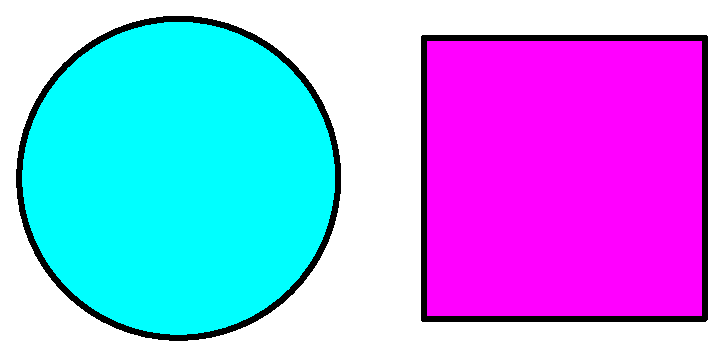
\includegraphics[width=0.4\textwidth]{square-circle}
  \caption{A square and a circle}
  \label{fig:square-circle}
\end{figure}

In maximus ante at metus vulputate congue. Sed eleifend ultrices tincidunt. Lorem ipsum dolor sit amet, consectetur adipiscing elit. Pr\ae{}sent quis rutrum elit. Nunc auctor nibh non sem consequat gravida. Nulla non dapibus metus. Cras viverra tempor nibh sit amet malesuada. Etiam non ante purus. M\ae{}cenas eleifend ultricies orci, ut fermentum erat suscipit elementum. Sed est libero, laoreet vel sodales ac, consectetur sed enim. Quisque hendrerit ac erat vit\ae{} posuere. Sed eros sapien, luctus ut justo lacinia, vestibulum sagittis lorem. Mauris porta dapibus dui, eu iaculis dolor faucibus id. 

%% }}} --- Section

%% ---------------------------
%% Bibliography and postamble
%% ---------------------------
%%%%%%%%%%%%%%%%%%%%%%%%%%%%%%%%%%%%%%%%%%%%%%%%%%%%%%%%%%%%%%%%%%%%%%%%%%
%% This file was autogenerated by PaperShell v2.6.1 on 2023-07-14 22:47:27
%% https://github.com/sylvainhalle/PaperShell
%% DO NOT EDIT!
%%%%%%%%%%%%%%%%%%%%%%%%%%%%%%%%%%%%%%%%%%%%%%%%%%%%%%%%%%%%%%%%%%%%%%%%%%
\bibliographystyle{elsarticle-num}

\section*{References}

\bibliography{paper}
%%%%%%%%%%%%%%%%%%%%%%%%%%%%%%%%%%%%%%%%%%%%%%%%%%%%%%%%%%%%%%%%%%%%%%%%%%
%% This file was autogenerated by PaperShell v2.6.1 on 2023-07-14 22:47:27
%% https://github.com/sylvainhalle/PaperShell
%% DO NOT EDIT!
%%%%%%%%%%%%%%%%%%%%%%%%%%%%%%%%%%%%%%%%%%%%%%%%%%%%%%%%%%%%%%%%%%%%%%%%%%
%% ---------------------------
%% If there is anything you would like to insert *after* the bibliography
%% (and *before* the \end{document} instruction), place it here
%% ---------------------------

% Nothing



\end{document}

%% :folding=explicit:wrap=soft:mode=latex: